\subsection{题目描述}
Electron in the finite square-well potential is, \( (V_0 = 10 \, \text{eV}, \, a = 0.2 \, \text{nm}) \)

\begin{figure}[h!]
    \centering
    \begin{minipage}{0.45\textwidth}
        \[
            V(x) =
            \begin{cases}
                V_0 & x \leq -a \quad \text{Region I}   \\
                0   & -a < x < a \quad \text{Region II} \\
                V_0 & x \geq a \quad \text{Region III}
            \end{cases}
        \]
    \end{minipage}
    \hspace{0.05\textwidth} % 控制间距
    \begin{minipage}{0.4\textwidth}
        \centering
        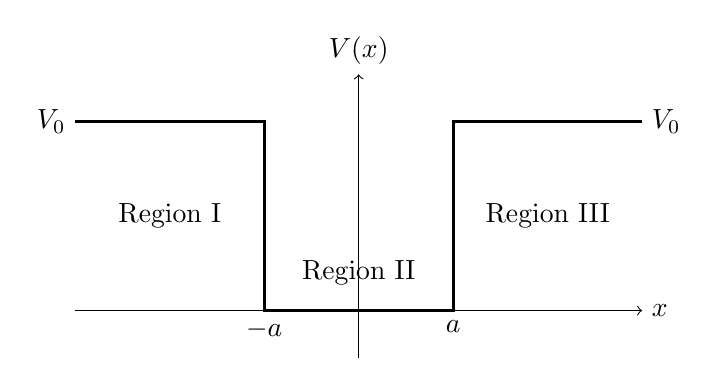
\begin{tikzpicture}[scale=1.2] % 缩放值按需调整
            % Potential well
            \draw[very thick] (-3,2) -- (-1,2) -- (-1,0) -- (1,0) -- (1,2) -- (3,2);
            \draw[->] (-3,0) -- (3,0) node[right] {$x$};
            \draw[->] (0,-0.5) -- (0,2.5) node[above] {$V(x)$};

            % Labels
            \node at (-2, 1) {Region I};
            \node at (0, 0.4) {Region II};
            \node at (2, 1) {Region III};

            \node[left] at (-3, 2) {$V_0$};
            \node[right] at (3, 2) {$V_0$};

            \node[below] at (-1,0) {$-a$};
            \node[below] at (1,0) {$a$};
        \end{tikzpicture}
    \end{minipage}
    \caption{Finite square-well potential and its corresponding mathematical expression.}
\end{figure}


Find the three lowest eigen states (\textbf{both} energies and wavefunctions).
\subsection{程序描述}
关于解析求解的方法,详情参见\textit{Griffiths}的量子力学教材,这里不再赘述。
主要是发现没时间了(大哭)

两种算法,一种针对本题的解析求解,即超越方程图解法:\texttt{./Codes/Problem_3/potential.py},另一种是数值求解:\texttt{./Codes/Problem_3/schrodinger.py},差分表示哈密顿矩阵,适用于更广泛的势能,偷懒都用Python实现了,不考虑效率还挺爽。

第二种方法是更普适的,有时间再推广研究研究:
有限差分法用于离散化薛定谔方程中的二阶导数项,便于在离散网格上构造哈密顿矩阵。在一维情况下,薛定谔方程为:


在离散网格上,每个点 \(x_i\) 的波函数值用 \(\psi_i = \psi(x_i)\) 表示,网格步长为 \(dx\)。二阶导数 \(\frac{d^2 \psi(x)}{dx^2}\) 在 \(x_i\) 处的离散近似为:

\[
    \frac{d^2 \psi(x)}{dx^2} \Big|_{x_i} \approx \frac{\psi_{i+1} - 2\psi_i + \psi_{i-1}}{dx^2}
\]

离散化后,整个系统的哈密顿矩阵 \(H\) 可以用三对角矩阵的形式表示。哈密顿矩阵的对角元和非对角元由动能项和势能项共同构成。对于每个网格点 \(x_i\):

1. 对角元 \(H[i, i]\) 包含动能项和势能项:
\[
    H[i, i] = -\frac{\hbar^2}{2m} \left( \frac{-2}{dx^2} \right) + V(x_i)
\]

2. 非对角元 \(H[i, i+1]\) 和 \(H[i, i-1]\) 只包含动能项:
\[
    H[i, i+1] = H[i, i-1] = -\frac{\hbar^2}{2m} \left( \frac{1}{dx^2} \right)
\]

最终,哈密顿矩阵 \(H\) 的形式为:

\[
    H = \begin{pmatrix}
        \ddots & \ddots                                  & \ddots                              &                                         & 0      \\
        \ddots & -\frac{2 \hbar^2}{2m dx^2} + V(x_{i-1}) & \frac{\hbar^2}{2m dx^2}             &                                         &        \\
        \ddots & \frac{\hbar^2}{2m dx^2}                 & -\frac{2 \hbar^2}{2m dx^2} + V(x_i) & \frac{\hbar^2}{2m dx^2}                 & \ddots \\
               &                                         & \frac{\hbar^2}{2m dx^2}             & -\frac{2 \hbar^2}{2m dx^2} + V(x_{i+1}) & \ddots \\
        0      &                                         &                                     & \ddots                                  & \ddots
    \end{pmatrix}
\]

这个三对角矩阵通过求解本征值问题,可以得到系统的能量特征值 \(E\) 以及对应的波函数 \(\psi\)。

\subsection{伪代码}

\begin{algorithm}[H]
    \caption{Intersection Calculation and Plotting of Functions}
    \label{alg:intersection_calculation}
    \KwIn{$z_0$ (float), $f_1(z)$, $f_2(z)$, $f_3(z)$}
    \KwOut{Intersections between $f_1(z)$ and $f_3(z)$, $f_2(z)$ and $f_3(z)$}

    $z_0 \gets 3.240175521$;\tcp*[r]{Initialize parameter $z_0$}
    $f_1(z) \gets \tan(z)$;\quad $f_2(z) \gets -\cot(z)$;\quad $f_3(z) \gets \sqrt{\left( \frac{z_0}{z} \right)^2 - 1}$;\tcp*[r]{Define functions}

    $z \in [0.1,\, z_0]$, $z \neq n \cdot \frac{\pi}{2},\ n \in \mathbb{Z}$;\tcp*[r]{Define valid range for $z$}

    $z \gets \text{Solve}(f_1(z) = f_3(z))$;\tcp*[r]{Find intersections of $f_1$ and $f_3$}
    $z \gets \text{Solve}(f_2(z) = f_3(z))$;\tcp*[r]{Find intersections of $f_2$ and $f_3$}

    $z \gets \text{Exclude}(z \approx n \cdot \frac{\pi}{2})$;\tcp*[r]{Exclude invalid solutions}

    $\text{Plot}(f_1(z), f_2(z), f_3(z));$\tcp*[r]{Plot all functions}
    $\text{Mark}(f_1(z) \cap f_3(z), \text{red});$\tcp*[r]{Mark valid intersections of $f_1$ and $f_3$}
    $\text{Mark}(f_2(z) \cap f_3(z), \text{green});$\tcp*[r]{Mark valid intersections of $f_2$ and $f_3$}

    $\text{Add axes, grid, title, legend};$\tcp*[r]{Customize the plot}

    \Return $\text{Intersections}(f_1(z), f_3(z), f_2(z), f_3(z));$\tcp*[r]{Return valid intersections}
\end{algorithm}

\begin{algorithm}[H]
    \caption{Finite Difference Solution of the Schrödinger Equation for a Finite Potential Well}
    \label{alg:schrodinger_equation}
    \KwIn{Constants $\hbar$, $m$, $V_0$, $a$, $N$, $L$}
    \KwOut{Bound state energy levels $E_{\text{bound}}$ (eV)}

    $N \gets 1000$,\quad $L \gets 10 \times 10^{-9}$;\tcp*[r]{Number of points and length scale}

    $dx \gets \dfrac{2L}{N - 1}$;\tcp*[r]{Spatial step size}
    $x_i \gets -L + i \cdot dx$, \quad for $i = 0$ to $N - 1$;\tcp*[r]{Generate grid points}

    $V_i \gets \begin{cases}
            -V_0, & \text{if } |x_i| \leq a                               \\ \tcp*[r]{Potential inside the well}
            0,    & \text{otherwise} \tcp*[r]{Potential outside the well}
        \end{cases}$\;

    \For{$i \gets 1$ \textbf{to} $N - 2$} {
        $H_{i,i-1} \gets 1$,\quad $H_{i,i} \gets -2$,\quad $H_{i,i+1} \gets 1$;\tcp*[r]{Fill the Hamiltonian matrix}
    }
    $H \gets H \cdot \dfrac{-(\hbar)^2}{2m\, dx^2}$\tcp*[r]{Construct Hamiltonian matrix $H$}
    $H_{i,i} \gets H_{i,i} + V_i$, \quad for $i = 0$ to $N - 1$;\tcp*[r]{Add potential to Hamiltonian}

    Find eigenvalues $E_n$ and eigenvectors $\psi_n$ such that $H \psi_n = E_n \psi_n$;\tcp*[r]{Solve eigenvalue problem}

    $E_{\text{bound}} \gets \{ E_n \mid E_n < 0,\ n > 0 \}$;\tcp*[r]{Select bound state energies}
    $\psi_{\text{bound}} \gets$ corresponding eigenvectors $\psi_n$;\tcp*[r]{Extract corresponding wavefunctions}

    $E_{\text{bound\_eV}} \gets E_{\text{bound}} / e$;\tcp*[r]{Convert energy to eV}

    $\psi_n \gets \psi_n / \sqrt{\sum_{i=0}^{N-1} |\psi_n(x_i)|^2\, dx}$, \quad for each $\psi_n$ in $\psi_{\text{bound}}$;\tcp*[r]{Normalize each wavefunction}

    Plot $\psi_n(x)$ shifted by $E_n$, \quad for each $E_n$ in $E_{\text{bound\_eV}}$;\tcp*[r]{Plot normalized wavefunctions}

    \Return $E_{\text{bound\_eV}}$;\tcp*[r]{Return bound state energies}
\end{algorithm}



\subsection{结果示例}
\begin{figure}[H]
    \centering
    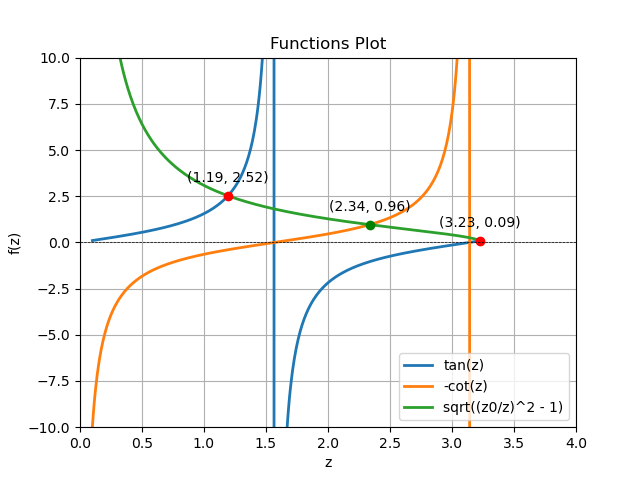
\includegraphics[width=1.0\textwidth]{Problem_3/Figs/3_fun.png}
    \caption{\texttt{potential.py}解析图解法}
    \label{fig:3_py_fun}
\end{figure}

\begin{figure}[H]
    \centering
    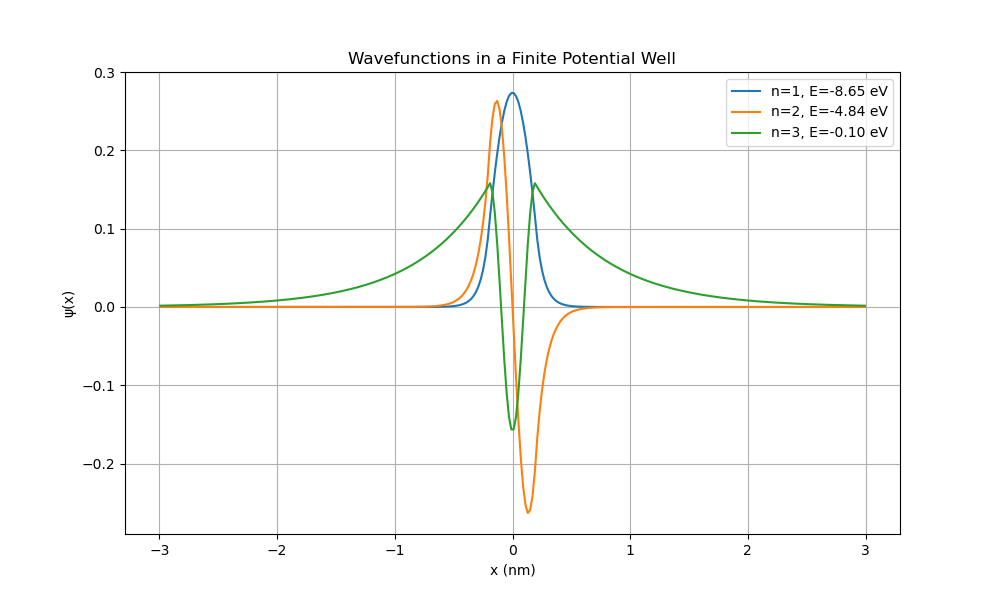
\includegraphics[width=1.0\textwidth]{Problem_3/Figs/3_diff.png}
    \caption{\texttt{schrodinger.py}数值差分法}
    \label{fig:3_py_diff}
\end{figure}